\section{Text Detection}

The penultimate stage of the pipeline is to crop each bib detection region and focus on the \gls{rbn} itself, as shown in \cref{fig:processing_pipeline:text_detection}. We attempted to train \frcnn{} using both the \gls{coco}-Text \citep{Veit:2016vj} and SynthText In The Wild \citep{Gupta:2016ws} datasets, following a similar process outlined in \cref{sec:processing_pipeline:bib_detection:deep_learning}. However, we found that---due to the wide variance of typeface samples within the \gls{coco}-Text dataset---\frcnn{} was only able to make reliable predictions on the SynthText dataset. Thus, we determined that \frcnn{} is suitable for text extraction given that it is trained on a dataset where text samples similar (i.e., the consistency of the synthetic words generated in the SynthText dataset made this possible).

Text detection used for two key purposes. Firstly, this helps to reduce false positives in the bib detection stage as if no text regions could be found, we assume the candidate region is not a bib image. Secondly, we use the largest text region on the bib found to pass feed into a text recognition engine. We explain this in the following section.

\begin{figure}[h]
  \centering
  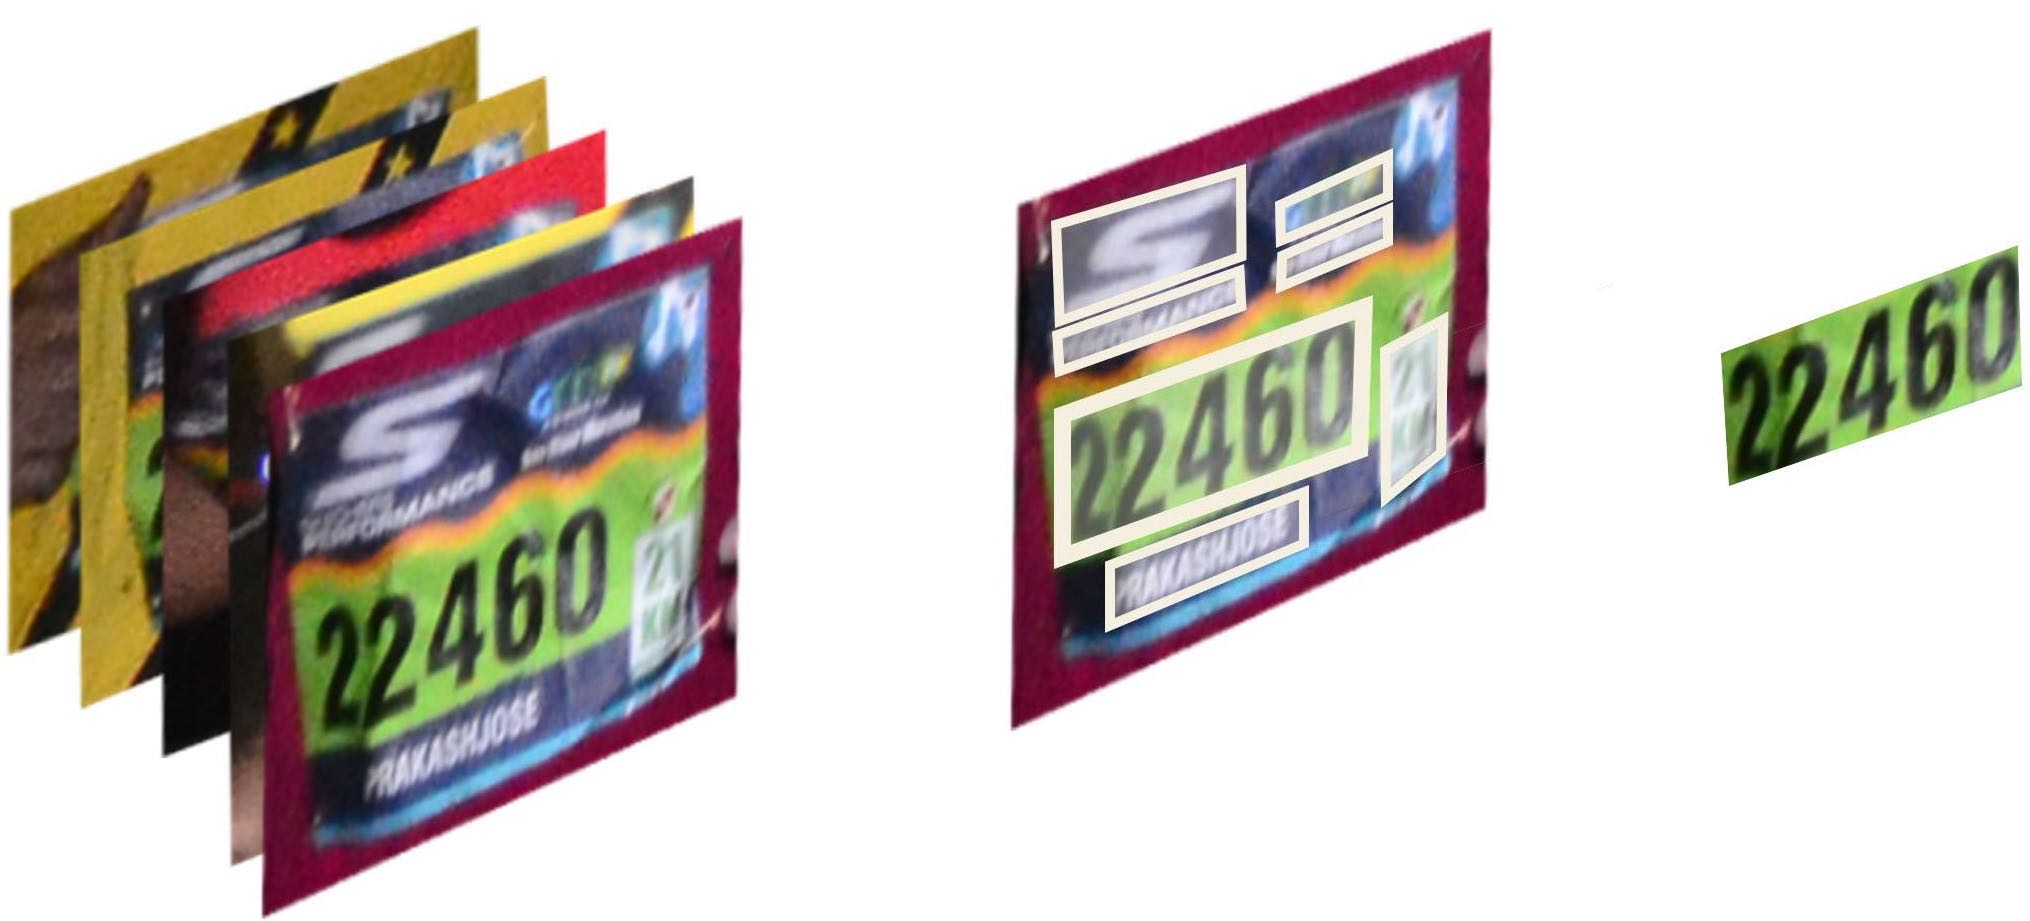
\includegraphics[width=\textwidth]{images/processing/text_process}
  \caption[Text region detection pipeline]{Text region detection. Detected bibs are cropped from the original image (left) and parsed through a text detection pipeline (middle). We select the candidate with the largest area and crop it (right).}
  \label{fig:processing_pipeline:text_detection}
\end{figure}

% DID USE THE Scene Text in The Wild....
% Tried to re-use FRCNN, but this network was not good enough. What dataset did we use, tried with COCO-Text but did not work. Tried with SynthText90k?
% Once we find the largest text region on the bib, we can then feed this into tesseract-4 alpha
